\documentclass[a4paper]{article} %Inicio de la clase
\usepackage[utf8]{inputenc} %Para los acentos
\usepackage[spanish]{babel}
\usepackage{amsmath}%Matematicas
\usepackage{amsfonts}
\usepackage{amssymb}
\usepackage{makeidx}
\usepackage{graphicx}%Para los graficos
\usepackage{fancyhdr}%Para los diseños de páginas
\usepackage{afterpage}%Paginas nuevas
\usepackage{verbatim}%Multicomentarios
\usepackage{listings}%Para insertar codigo
\usepackage{lmodern}
\usepackage{multicol}%Para poner columnas en el documento
\usepackage{kpfonts}
\usepackage{color}

\usepackage{fourier}%Series avanzadas de Fourier
\usepackage[left=2cm,right=2cm,top=2cm,bottom=2cm]{geometry}
\author{Gonzalez Hinojosa Emiliano}%Autor

%Definimos los colores para el codigo Python
\definecolor{fondo}{rgb}{0.43, 0.5, 0.5}
\definecolor{palabrasClave}{rgb}{0.4, 1.0, 0.0}
\definecolor{comentarios}{rgb}{0.29, 0.33, 0.13}
\definecolor{lineas}{rgb}{ 0.0, 0.5, 0.0}
\definecolor{cadenas}{rgb}{1.0, 0.0, 0.22}

\lstset{ 
  backgroundcolor=\color{white},   % Indica el color de fondo; necesita que se añada \usepackage{color} o \usepackage{xcolor}
  basicstyle=\footnotesize,        % Fija el tamaño del tipo de letra utilizado para el código
  breakatwhitespace=false,         % Activarlo para que los saltos automáticos solo se apliquen en los espacios en blanco
  breaklines=true,                 % Activa el salto de línea automático
  commentstyle=\color{comentarios},% Estilo de los comentarios
  frame=single,	                   % Añade un marco al código
  keepspaces=false,                 % Es útil para mantener la indentación del código(puede necesitar columns=flexible).
  keywordstyle=\color{palabrasClave},% estilo de las palabras clave
  language=Python,                 % El lenguaje del código
  numbers=left,                    % Posición de los números de línea (none, left, right).
  numbersep=5pt,                   % Distancia de los números de línea al código
  numberstyle=\small\color{lineas},% Estilo para los números de línea
  rulecolor=\color{lineas},         % Si no se activa, el color del marco puede cambiar en los saltos d  showspaces=true,                
  stepnumber=1,                    % Muestra solamente los números de línea que corresponden a cada salto. 
  stringstyle=\color{blue},     % Estilo de las cadenas de texto
  title=\lstname                   % muestra el nombre de los ficheros incluidos al utilizar \lstinputlisting; 
}

\begin{document} 	
	\begin{titlepage}

		\begin{center}
		\vspace{1cm}
		
		\vspace{0.7cm}
		\textbf{\LARGE{INSTITUTO POLITECNICO NACIONAL}}\\
		\vspace{0.5cm}
		\textit{\Large{Escuela Superior de Cómputo}}\\
		\vspace{0.5cm}		
		\begin{figure}[ht]
			\begin{center}
				
\includegraphics[width=5cm,height=5cm]{IPNLOGO.jpg}				
			\end{center} 
		\end{figure}
		
		%Dejaremos espacios		
		\vspace{1.3cm}
		\textbf{\LARGE{Análisis De Algoritmos}}\\
		\vspace{1cm}		
		\textbf{\Large{ Práctica 9}}\\
		
		\textit{--> \textbf{Programación Dinámica:} Heap Sort, Counting Sort and Radix Sort. <--}\\
		
		\vspace{2cm}
		\textbf{\Large{Emiliano Gonzalez Hinojosa}}\\		
		\vspace{0.3cm}
		\textit{\Large{metalica\_el\_01@hotmail.com}}\\
		\vspace{0.5cm}
		\textit{\Large{Semestre 2018}}\\
		\vspace{0.2cm}
		\textbf{\Large{Grupo 3CV2}}\\
		\vspace{0.5cm}
		
		
		\vspace{8cm}

		\rule{170mm}{0.8mm}\\
		
		\end{center}
	\end{titlepage}
	
	
	\part{Contenido}
	
	\section{Introducción}
		\subsection{ Finalidad y Objetivo.}
		
	\section{Conceptos Básicos}
		\subsection{Counting Sort}
		\subsection{Heap Sort}
		\subsection{Radix Sort}
		
	\section{Experimentación}
		\subsection{Counting Sort}
		\subsection{Heap Sort}
		\subsection{Radix Sort}			
			
	\section{Conclusiones}
		\subsection{Opinion Personal.}	

	\section{Bibliografía}
		\subsection{Libros Recomendados.}	
	
	
	\afterpage{\newpage}
	\newpage
	
	%INTRODUCCION
	\section*{Introducción}
		\subsection*{Finalidad y Objetivo}		
		Éste reporte tiene la finalidad de mostrar y dar a conocer la importancia de funcionamiento de los algoritmos que 					comúnmente el alumno desarrolla en clase.\\ Así mismo nos da algunos conceptos que nos ayudaran a comprender como es que 			la máquina (el compilador) cumple su funcionamiento y, nos muestra el costo computacional que se tiene al desarrollar 				ciertas prácticas en la vida cotidiana.
		
	\section*{Conceptos Básicos}
		\subsection*{Counting Sort}
		El ordenamiento por cuentas (counting sort en inglés) es un algoritmo de ordenamiento en el que se cuenta el número de elementos de cada clase para luego ordenarlos. Sólo puede ser utilizado por tanto para ordenar elementos que sean contables (como los números enteros en un determinado intervalo, pero no los números reales, por ejemplo).

El primer paso consiste en averiguar cuál es el intervalo dentro del que están los datos a ordenar (valores mínimo y máximo). Después se crea un vector de números enteros con tantos elementos como valores haya en el intervalo [mínimo, máximo], y a cada elemento se le da el valor 0 (0 apariciones). Tras esto se recorren todos los elementos a ordenar y se cuenta el número de apariciones de cada elemento (usando el vector que hemos creado). Por último, basta con recorrer este vector para tener todos los elementos ordenados.
		\subsection*{Limitaciones}
		Sólo ordena números enteros, no vale para ordenar cadenas y es desaconsejable para ordenar números decimales. Teóricamente se puede, pero debería recrear en la matriz auxiliar tantas posiciones como decimales quepan entre 2 números consecutivos, si se restringe a 1 o 2 decimales podría ser asequible un número mayor de decimales puede llegar a suponer una memoria auxiliar impracticable.\\
		Otra limitación (por ineficiencia) incluso con números enteros es cuando el rango entre el mayor y el menor es muy grande. 

		\begin{figure}[ht]
			\begin{center}
				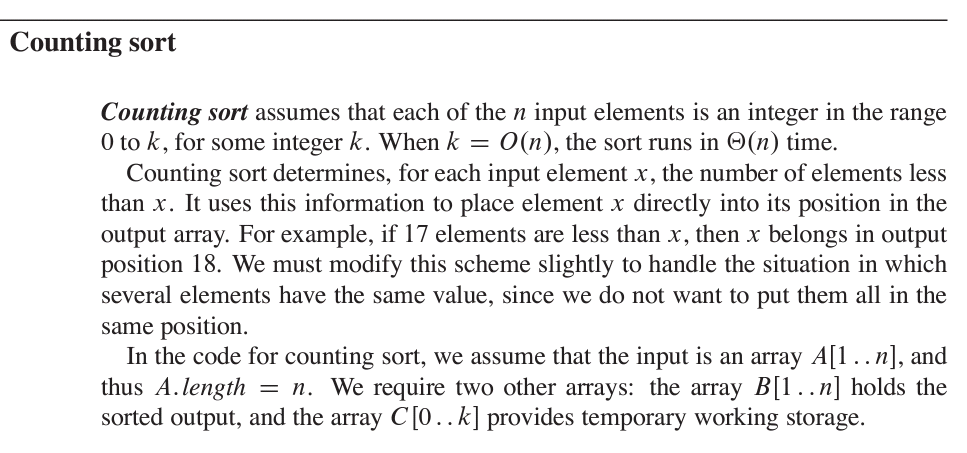
\includegraphics[width=\textwidth,height=60mm]{Imagenes/countingsort/counting01.png}				
			\end{center} 
		\end{figure}
		\afterpage{\newpage}
		\newpage
		\begin{figure}[ht]
			\begin{center}
				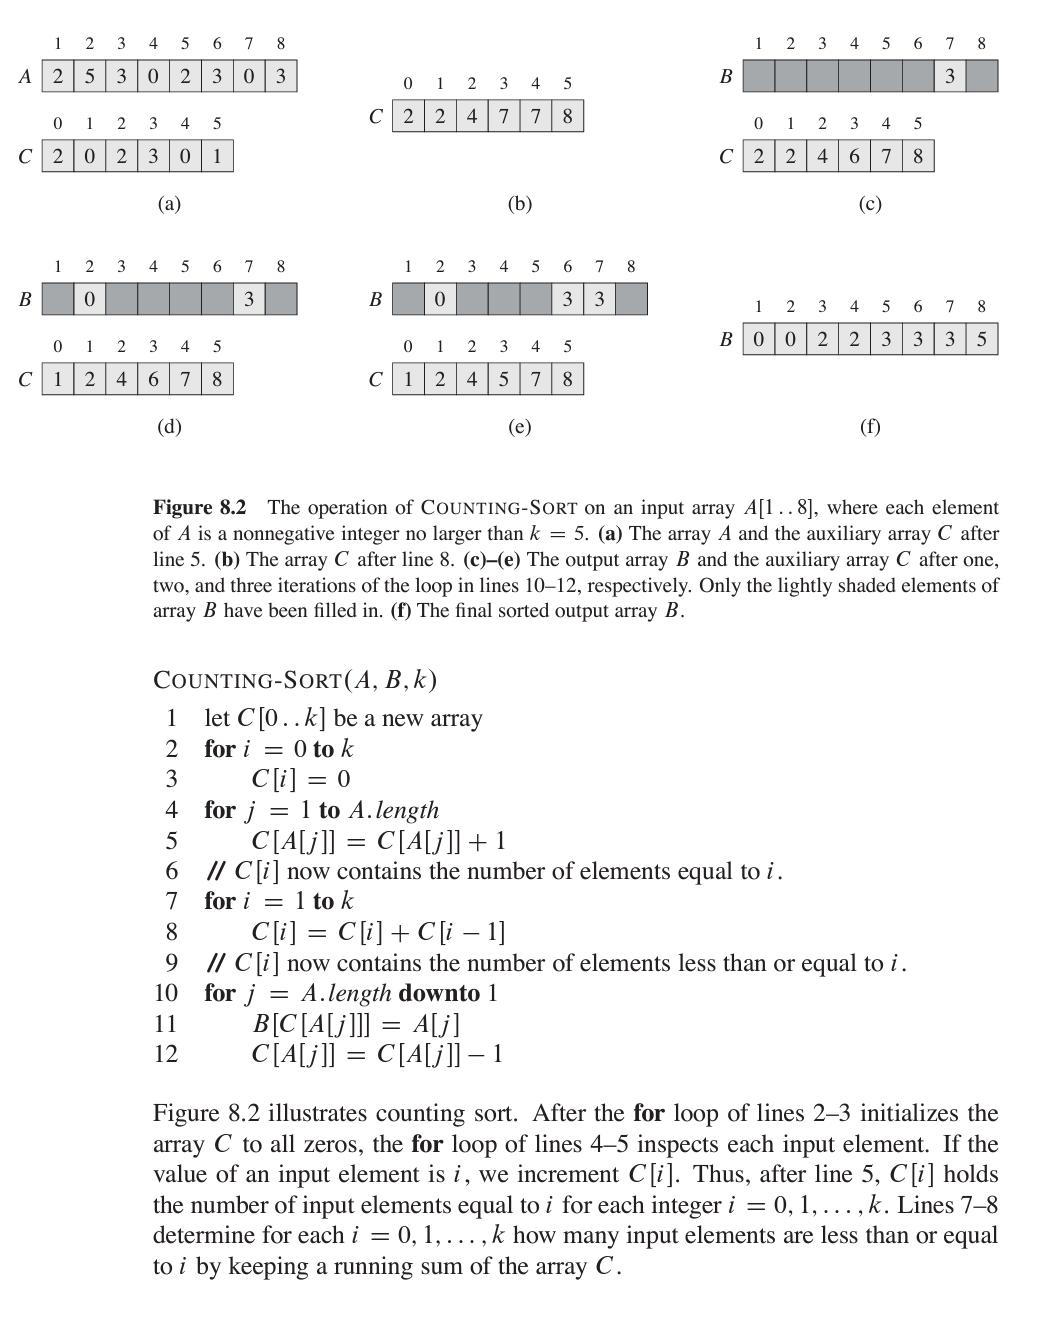
\includegraphics[width=\textwidth,height=190mm]{Imagenes/countingsort/counting02.png}				
			\end{center} 
		\end{figure}
		\afterpage{\newpage}
		\newpage
		
		\subsection*{Heap Sort}
		Animación mostrando el funcionamiento del heapsort.
		El ordenamiento por montículos (heapsort en inglés) es un algoritmo de ordenamiento no recursivo, no estable.\\ \\
		Este algoritmo consiste en almacenar todos los elementos del vector a ordenar en un montículo (heap), y luego extraer el nodo que queda como nodo raíz del montículo (cima) en sucesivas iteraciones obteniendo el conjunto ordenado. Basa su funcionamiento en una propiedad de los montículos, por la cual, la cima contiene siempre el menor elemento (o el mayor, según se haya definido el montículo) de todos los almacenados en él. El algoritmo, después de cada extracción, recoloca en el nodo raíz o cima, la última hoja por la derecha del último nivel. Lo cual destruye la propiedad heap del árbol. Pero, a continuación realiza un proceso de "descenso" del número insertado de forma que se elige a cada movimiento el mayor de sus dos hijos, con el que se intercambia. Este intercambio, realizado sucesivamente "hunde" el nodo en el árbol restaurando la propiedad montículo del árbol y dejándo paso a la siguiente extracción del nodo raíz.	
		
		\afterpage{\newpage}
		\newpage		

		\subsection*{Radix Sort}
		
		En informática, el ordenamiento Radix (radix sort en inglés) es un algoritmo de ordenamiento que ordena enteros procesando sus dígitos de forma individual. Como los enteros pueden representar cadenas de caracteres (por ejemplo, nombres o fechas) y, especialmente, números en punto flotante especialmente formateados, radix sort no está limitado sólo a los enteros.\\
		Radix sort LSD procesa las representaciones de enteros empezando por el dígito menos significativo y moviéndose hacia el dígito más significativo. Radix sort MSD trabaja en sentido contrario.\\
		\begin{figure}[ht]
			\begin{center}
				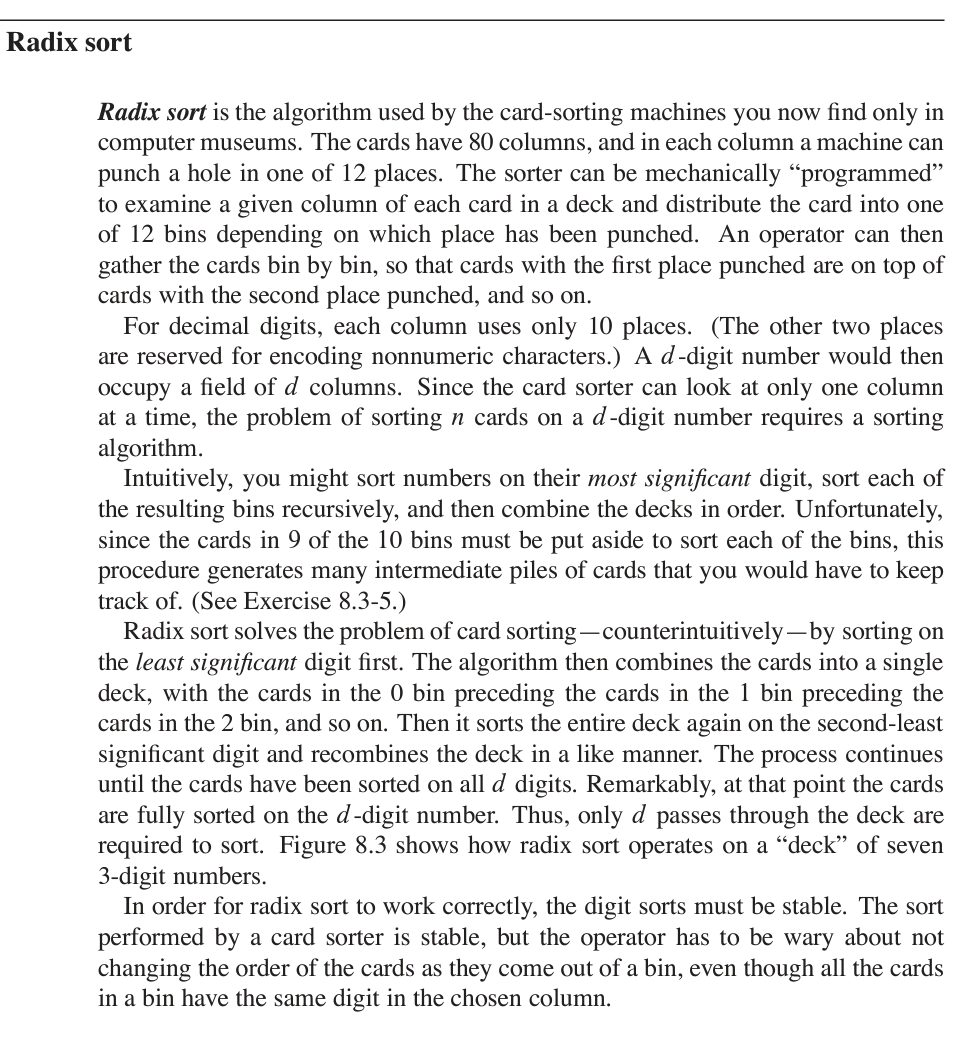
\includegraphics[width=\textwidth,height=160mm]{Imagenes/radixsort/radix01.png}				
			\end{center} 
		\end{figure}
		\afterpage{\newpage}
		\newpage
		\begin{figure}[ht]
			\begin{center}
				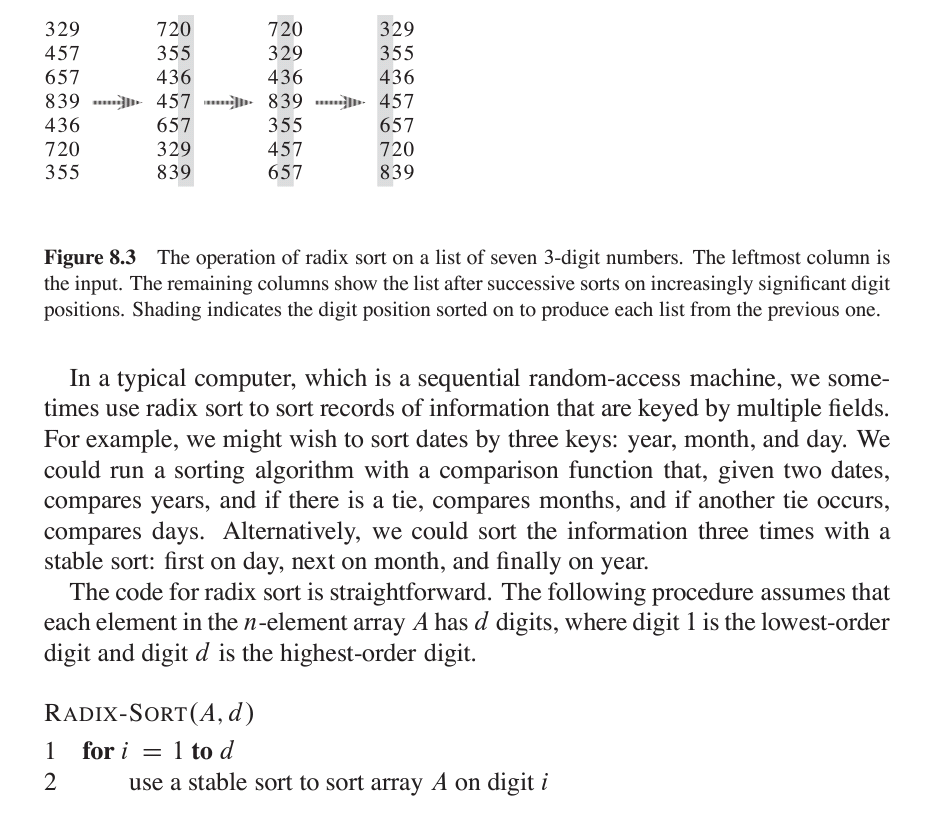
\includegraphics[width=\textwidth,height=180mm]{Imagenes/radixsort/radix02.png}				
			\end{center} 
		\end{figure}
		\afterpage{\newpage}
		\newpage
			
			
	\section*{Experimentación}
		\textbf{Para la parte de la experimentación los programas fueron desarrollados en JAVA y las clases fueron las siguientes: Practica8.java(La Princiapal), CountingSort.java, HeapSort.java y RadixSort.java}\\
		\subsection*{Counting Sort}
			\textbf{ A continuación se mostrará el código:}
			\lstinputlisting[language=Java]{CountingSort.java}
			\afterpage{\newpage}
			\newpage			
		\subsection*{Heap Sort}
			\textbf{ A continuación se mostrará el código:}
			\lstinputlisting[language=Java]{HeapSort.java}
			\afterpage{\newpage}
			\newpage
		\subsection*{Radix Sort}	
			\textbf{ A continuación se mostrará el código:}
			\lstinputlisting[language=Java]{RadixSort.java}	
			\afterpage{\newpage}
			\newpage		
		\subsection*{Función Principal}	
			\textbf{ A continuación se mostrará el código:}
			\lstinputlisting[language=Java]{Practica9.java}				
			\afterpage{\newpage}
			\newpage		
	\section*{Conclusiones}
		\subsection*{Opinion Personal.}
		\vspace{0.5cm}
		Sin duda el poder analizar algoritmos de forma recursiva no es algo trivial. A veces es un poco complicado poder definir la funció y lejos de eso, lo que se complica es la condicion de paro ya que sin esta no podemos tener una certeza de que lo que estamos planteando como solucion es correcto.\\
		De igual forma, a veces algunos algoritmos recursivos se comportan de diferente forma para los diferentes valores de los argumentos.
		
	
	\afterpage{\newpage}
	\newpage		
	\section*{Bibliografía}
		\subsection*{Libros Recomendados}
		[ 1 ] Baase and Van Gelder.  ”Computer Algorithms:  Introduction to Design and Analysis”.  Addison-                						  Wesley.
		 
		[ 2 ] Thomas H. Cormen.  ”Introduction to Algorithms”.  The MIT press.
		
\end{document}